% !TEX TS-program = XeLaTeX
% use the following command:
% all document files must be coded in UTF-8
\documentclass[spanish]{textolivre}
% build HTML with: make4ht -e build.lua -c textolivre.cfg -x -u article "fn-in,svg,pic-align"

\journalname{Texto Livre}
\thevolume{15}
%\thenumber{1} % old template
\theyear{2022}
\receiveddate{\DTMdisplaydate{2022}{5}{10}{-1}} % YYYY MM DD
\accepteddate{\DTMdisplaydate{2022}{6}{25}{-1}}
\publisheddate{\DTMdisplaydate{2022}{9}{03}{-1}}
\corrauthor{Susan Rivera Robles}
\articledoi{10.35699/1983-3652.2022.39657}
%\articleid{NNNN} % if the article ID is not the last 5 numbers of its DOI, provide it using \articleid{} commmand 
% list of available sesscions in the journal: articles, dossier, reports, essays, reviews, interviews, editorial
\articlesessionname{articles}
\runningauthor{Rivera-Robles et al.} 
%\editorname{Leonardo Araújo} % old template
\sectioneditorname{Hugo Heredia Ponce}
\layouteditorname{Daniervelin Pereira}

\title{Cambios en la autopercepción tecnológica de los docentes en contexto de pandemia}
\othertitle{Mudanças na autopercepção tecnológica de professores no contexto de uma pandemia}
\othertitle{Changes in the technological self-perception of teachers in the context of a pandemic}
% if there is a third language title, add here:
%\othertitle{Artikelvorlage zur Einreichung beim Texto Livre Journal}

\author[1]{Susan Rivera-Robles \orcid{0000-0001-6086-4992} \thanks{Email: \href{mailto:srivera@ucsc.cl}{srivera@ucsc.cl}}}
\author[2]{Pedro Salcedo-Lagos \orcid{0000-0002-1741-714X} \thanks{Email: \href{mailto:psalcedo@udec.cl}{psalcedo@udec.cl}}}
\author[2]{Carolina Fernández-Chávez \orcid{0000-0002-8115-1374} \thanks{Email: \href{mailto:carofernandezc@udec.cl}{carofernandezc@udec.cl}}}
\author[3]{María Graciela Badilla-Quintana \orcid{0000-0002-1317-9228} \thanks{Email: \href{mailto:mgbadilla@ucsc.cl}{mgbadilla@ucsc.cl}}}
\affil[1]{Universidad Católica de la Santísima Concepción, Doctorado en Ciencias de la Educación, Concepción, Chile.}
\affil[2]{Universidad de Concepción, Facultad de Educación, Concepción, Chile.}
\affil[3]{Universidad Católica de la Santísima Concepción, Centro de Investigación en Educación y Desarrollo, Concepción, Chile.}

\addbibresource{article.bib}
% use biber instead of bibtex
% $ biber article

% used to create dummy text for the template file
\definecolor{dark-gray}{gray}{0.35} % color used to display dummy texts
\usepackage{lipsum}
\SetLipsumParListSurrounders{\colorlet{oldcolor}{.}\color{dark-gray}}{\color{oldcolor}}

% used here only to provide the XeLaTeX and BibTeX logos
\usepackage{hologo}

% if you use multirows in a table, include the multirow package
\usepackage{multirow}

% provides sidewaysfigure environment
\usepackage{rotating}

% CUSTOM EPIGRAPH - BEGIN 
%%% https://tex.stackexchange.com/questions/193178/specific-epigraph-style
\usepackage{epigraph}
\renewcommand\textflush{flushright}
\makeatletter
\newlength\epitextskip
\pretocmd{\@epitext}{\em}{}{}
\apptocmd{\@epitext}{\em}{}{}
\patchcmd{\epigraph}{\@epitext{#1}\\}{\@epitext{#1}\\[\epitextskip]}{}{}
\makeatother
\setlength\epigraphrule{0pt}
\setlength\epitextskip{0.5ex}
\setlength\epigraphwidth{.7\textwidth}
% CUSTOM EPIGRAPH - END

% LANGUAGE - BEGIN
% ARABIC
% for languages that use special fonts, you must provide the typeface that will be used
% \setotherlanguage{arabic}
% \newfontfamily\arabicfont[Script=Arabic]{Amiri}
% \newfontfamily\arabicfontsf[Script=Arabic]{Amiri}
% \newfontfamily\arabicfonttt[Script=Arabic]{Amiri}
%
% in the article, to add arabic text use: \textlang{arabic}{ ... }
%
% RUSSIAN
% for russian text we also need to define fonts with support for Cyrillic script
% \usepackage{fontspec}
% \setotherlanguage{russian}
% \newfontfamily\cyrillicfont{Times New Roman}
% \newfontfamily\cyrillicfontsf{Times New Roman}[Script=Cyrillic]
% \newfontfamily\cyrillicfonttt{Times New Roman}[Script=Cyrillic]
%
% in the text use \begin{russian} ... \end{russian}
% LANGUAGE - END

% EMOJIS - BEGIN
% to use emoticons in your manuscript
% https://stackoverflow.com/questions/190145/how-to-insert-emoticons-in-latex/57076064
% using font Symbola, which has full support
% the font may be downloaded at:
% https://dn-works.com/ufas/
% add to preamble:
% \newfontfamily\Symbola{Symbola}
% in the text use:
% {\Symbola }
% EMOJIS - END

% LABEL REFERENCE TO DESCRIPTIVE LIST - BEGIN
% reference itens in a descriptive list using their labels instead of numbers
% insert the code below in the preambule:
%\makeatletter
%\let\orgdescriptionlabel\descriptionlabel
%\renewcommand*{\descriptionlabel}[1]{%
%  \let\orglabel\label
%  \let\label\@gobble
%  \phantomsection
%  \edef\@currentlabel{#1\unskip}%
%  \let\label\orglabel
%  \orgdescriptionlabel{#1}%
%}
%\makeatother
%
% in your document, use as illustraded here:
%\begin{description}
%  \item[first\label{itm1}] this is only an example;
%  % ...  add more items
%\end{description}
% LABEL REFERENCE TO DESCRIPTIVE LIST - END


% add line numbers for submission
%\usepackage{lineno}
%\linenumbers
\usepackage{siunitx}
\sisetup{output-decimal-marker={,}}

\begin{document}
\maketitle

\begin{polyabstract}
\begin{abstract}
Este estudio relaciona los cambios en la autopercepción de los docentes en contexto de pandemia con las necesidades curriculares sugeridas desde el Ministerio de Educación de Chile. El objetivo fue analizar los objetivos de las priorizaciones curriculares y el grado de autovaloración sobre la integración de las tecnologías de profesores en contexto de prepandemia y pandemia. El estudio tuvo un carácter analítico, interpretativo y comparativo. Se seleccionaron 178 docentes, se les aplicó un cuestionario TPACK en diciembre de 2020 y enero de 2021, además se seleccionaron cuatro asignaturas para realizar nubes de palabras a partir de sus objetivos priorizados. Se analizaron los resultados de forma descriptiva, comparativa con otra muestra tomada en 2018 y entre otros grupos demográficos. Los resultados revelaron diferencias significativas en varios componentes del TPACK (TK, PK, PCK, TCK y TPK) de los docentes. Se concluye que los docentes en contexto de pandemia se auto perciben con mayor conocimiento tecnológico, pero menor conocimiento pedagógico y de contenido que los docentes en contexto de prepandemia, no coincidiendo con las necesidades curriculares en este periodo, donde se necesita mayor manejo de contenido y pedagógico para contextualizar el aprendizaje.

\keywords{TPACK \sep COVID-19 \sep Educación remota \sep Priorización curricular \sep Percepción docente}
\end{abstract}

\begin{portuguese}
\begin{abstract}
Este estudo relaciona as mudanças na autopercepção dos professores no contexto de uma pandemia com as necessidades curriculares sugeridas pelo Ministério da Educação do Chile. O objetivo foi analisar os objetivos das prioridades curriculares e o grau de autoavaliação sobre a integração das tecnologias docentes no contexto de pré-pandemia e pandemia. O estudo teve natureza analítica, interpretativa e comparativa. Foram selecionados 178 professores, a quem foi aplicado um questionário TPACK em dezembro de 2020 e janeiro de 2021. Além disso, quatro disciplinas foram selecionadas para fazer nuvens de palavras com base em seus objetivos priorizados. Os resultados foram analisados de forma descritiva, comparativamente com outra amostra realizada em 2018 e entre outros grupos demográficos. Os resultados revelaram diferenças significativas em vários componentes do TPACK (TK, PK, PCK, TCK e TPK) dos professores. Conclui-se que os professores em contexto de pandemia percebem-se como detentores de maior conhecimento tecnológico, mas menos conhecimento pedagógico e de conteúdo do que professores em contexto pré-pandemia, não coincidindo com as necessidades curriculares nesse período, quando é necessária uma maior gestão de conteúdos e pedagogia para contextualizar a aprendizagem.

\keywords{TPACK \sep COVID-19 \sep Ensino remoto \sep Priorização curricular \sep Percepção do professor}
\end{abstract}
\end{portuguese}

\begin{english}
\begin{abstract}
This study relates the changes in the self-perception of teachers in the context of pandemic with the curricular needs suggested by the Chilean Ministry of Education. The objective was to analyze the objectives of the curricular prioritizations and the degree of self-assessment on the integration of technologies of teachers in pre-pandemic and pandemic contexts. The study was analytical, interpretative and comparative. A total of 178 teachers were selected, a TPACK questionnaire was applied to them in December 2020 and January 2021, and four subjects were selected for word clouds based on their prioritized objectives. Results were analyzed descriptively, comparatively with another sample taken in 2018 and among other demographic groups. The results revealed significant differences in several TPACK components (TK, PK, PCK, TCK, and TPK) of teachers. It is concluded that teachers in pandemic context self-perceive themselves with greater technological knowledge, but less pedagogical and content knowledge than teachers in pre-pandemic context, not coinciding with the curricular needs in this period, where greater content and pedagogical management is needed to contextualize learning.

\keywords{TPACK \sep COVID-19 \sep Remote education \sep Curricular prioritization \sep Teacher perception}
\end{abstract}
\end{english}
% if there is another abstract, insert it here using the same scheme
\end{polyabstract}

\section{Introducción}\label{sec-intro}
El SARS-COV2 ha impactado a todo el mundo desde diciembre de 2019 hasta la fecha, por lo que el ámbito educativo ha tenido que dar un vuelco en la metodología de enseñanza. La paralización de clases presenciales en marzo de 2020 fue una de las medidas tomadas por el gobierno chileno para evitar los contagios en la población \cite{unesco_impacto_2020}, seguidamente el Ministerio de Educación de Chile (MINEDUC) entregó las indicaciones para continuar con el año escolar mediante clases remotas, donde la priorización curricular fue clave en este proceso \cite[p. 6-27]{unidad_de_curriculum_y_evaluacion_uce_fundamentacion_2020a}. Basado en la adecuación curricular y el decreto 83/2015 \cite[p. 10-14]{ministerio_de_educacion_mineduc_orientaciones_2017} se priorizan objetivos necesarios para que el estudiantado pudiera continuar al siguiente nivel escolar, apuntando a tres principios básicos: seguridad, flexibilidad y equidad, a los cuales se suma el principio que define a la educación de calidad como aquella que es capaz de estructurar los procesos de enseñanza y aprendizaje de forma variada y flexible \cite[p. 16]{ministerio_de_educacion_mineduc_orientaciones_2017}. El decreto 83/2015 establece las regularidades para la adecuación curricular en la educación inclusiva. Mediante este decreto se detallan los aprendizajes que deben fomentarse para el desarrollo integral de los estudiantes. En este contexto, el Ministerio destaca que la alfabetización digital y el manejo de las TIC (Tecnologías de la Información y el Conocimiento) es fundamental para resguardar el aprendizaje escolar por esta razón es necesario que los docentes tengan manejo tecnológico en sus áreas respectivas \cite[p. 8]{unidad_de_curriculum_y_evaluacion_uce_fundamentacion_2020a}.

La priorización curricular reordena los objetivos en dos grupos, Nivel 1: objetivos imprescindibles para la continuidad de estudios y Nivel 2: objetivos significativos e integradores para ampliar el currículum. La implementación y evaluación de este currículum transitorio debe adecuarse al contexto de cada institución, por lo que el rol de la escuela y de los docentes, es fundamental para llevar a cabo este desafío \cite[p. 8]{unidad_de_curriculum_y_evaluacion_uce_fundamentacion_2020a}. Por lo tanto, los docentes deben tener cuidado de no aplicar la priorización tal como viene prescrita. 

La pandemia dejó en evidencia las brechas económicas, manifestándose en la escases de recursos digitales básicos como computadores e internet para todos los estudiantes \cite[p. 3]{quiroz_reyes_pandemia_2020}. Así lo afirma el estudio de \textcite[p. 8]{anderete_schwal_confinamiento_2022} donde el aislamiento agravó la desigualdad entre instituciones educativas públicas y privadas. \textcite[p. 6]{dussel_escuela_2020} indica que surgieron cuatro tensiones al realizar clases a distancia en tiempos de pandemia:
\begin{enumerate*}[label=(\arabic*)]
\item la tensión de las desigualdades, 
\item la individualización de las pedagogías, 
\item la domesticación de la escuela, y 
\item la pérdida de los espacios de conversación. 
\end{enumerate*}
Adicionalmente, nos encontramos con el poco uso de TIC por parte de los docentes, quienes utilizan recursos digitales mayoritariamente para la preparación de sus clases en lugar de implementarlas en el aula \cite{agencia_de_calidad_de_la_education_ace_estudio_2018,ibieta_role_2017}. Conocer la percepción de los docentes es indispensable para realizar un cambio en la metodología de trabajo y para que el Mineduc pueda entregar una orientación adecuada hacia la alfabetización digital \cite[p. 25]{agencia_de_calidad_de_la_educacion_ace_estudio:_2020}.

Una manera de conocer la percepción de los docentes respecto a su conocimiento disciplinar, pedagógico y tecnológico, es por medio del modelo de Conocimiento Tecnológico Pedagógico del Contenido (TPACK) \cite[p. 1]{thompson_editors_2007}. Este marco referencial cuenta con un cuestionario creado por \textcite{schmidt_technological_2009} y adaptado al español por \textcite{cabero_formacion_2014}. 

Con respecto a lo anterior, existen diferentes estudios que demuestran que los profesores se perciben con un alto manejo tecnológico \cite{arancibia_herrera_percepcion_2018,ministerio_de_educacion_mineduc_docentes_2016,rios_ariza_valoracion_2018}. Sin embargo, hay evidencias que indican que los docentes tienen una baja competencia TIC \cite{agencia_de_calidad_de_la_educacion_ace_estudio:_2020,canales_politica_2017,agencia_de_calidad_de_la_education_ace_estudio_2018,silva_teachers_2019}. En contexto de pandemia, el conocimiento y la autopercepción de los profesionales respecto al uso de las tecnologías pudiese haber cambiado. Considerando que estos factores deben responder a las necesidades requeridas en los objetivos priorizados, resulta interesante estudiar ambos aspectos dado que los docentes han estado expuestos a nuevas experiencias tecnológicas durante la pandemia \cite[p. 158]{santi_teachers_2020}, además, se ha detectado escasa investigación sobre estas temáticas. 

Este estudio toma el TPACK de profesores chilenos antes de la pandemia, con una muestra tomada en 2018, y lo compara con el TPACK en contexto de pandemia para evidenciar si existen cambios significativos. Además, se centra en dar a conocer los resultados obtenidos a partir del cuestionario TPACK y las nubes de palabras donde se analizan las necesidades de los objetivos priorizados dictados por el MINEDUC. 

Consecuentemente, esta investigación se centra en resolver tres preguntas: 

\begin{enumerate}
    \item ¿Cuál es la validez del instrumento diagnóstico del modelo TPACK para docentes chilenos en contexto de pandemia?
    \item ¿Cómo es el grado de autovaloración sobre la integración de las tecnologías de los profesores chilenos en el contexto de pandemia?
    \item ¿Cuál es el cambio en la autopercepción de los docentes chilenos en contexto de pandemia respecto a los docentes en contexto de prepandemia, en cuanto a tecnología en educación, y su relación con las priorizaciones curriculares?
\end{enumerate}

\section{Antecedentes Teóricos}\label{sec-normas}
\subsection{Integración curricular de las TIC}
El docente del siglo XXI debe ser un facilitador de aprendizajes teniendo manejo de las TIC y de la integración didáctica y pedagógica de estos recursos \cite{del_moral_perez_formacion_2010,hernandez_nuevas_2018}. La sociedad exige docentes que manejen e integren las TIC en sus prácticas habituales para que los estudiantes logren altas competencias tecnológicas \cite{cozar_gutierrez_creando_2015,unesco_padroes_2009}, siendo el profesor el responsable de facilitar y diseñar actividades que propicien el manejo tecnológico \cite{cejas_leon_competencias_2016,unesco_uso_2013}. 

Sánchez (2002, p. 5) define las TIC como un proceso de integración de tecnologías en el quehacer pedagógico, incorporándolo en las planificaciones y actividades con un fin curricular explícito, es decir, con un objetivo de aprendizaje. Pese a esto, los docentes tienden a utilizar los recursos tecnológicos para transmitir conocimientos sin integrar competencias pedagógicas y tecnológicas \cite{cabero_formacion_2014,suarez_rodriguez_competencias_2013}.
Por lo anterior, es necesario que el docente integre los saberes, el contexto y el manejo de TIC en su desarrollo profesional \cite{cejas_leon_competencias_2016,sampaio_ensinar_2013}, haciendo de las tecnologías parte del currículum y no como un recurso aparte \cite[p. 1]{sanchez_integracion_2002}. Un modelo teórico que permite esta integración es el modelo TPACK.

\subsection{Modelo TPACK}\label{sec-conduta}
En el año 2006 se introdujo el término Conocimiento Tecnológico Pedagógico del Contenido como el concepto que describe los conocimientos necesarios para la enseñanza de las tecnologías \cite{mishra_technological_2006}. Este concepto se basa en los fundamentos de \textcite{shulman_those_1986,shulman_knowledge_1987} sobre el conocimiento pedagógico del contenido (PCK), los cuales se relacionan con conocimientos tecnológicos \cite{mishra_technological_2007}. El modelo TPACK consta de tres categorías principales: conocimiento de contenido (CK), conocimiento pedagógico (PK) y conocimiento tecnológico (TK). La combinación de estas categorías da como resultado cuatro categorías adicionales: conocimiento de contenido pedagógico (PCK), conocimiento pedagógico tecnológico (TPK), conocimiento de contenido tecnológico (TCK) y conocimiento de contenido pedagógico tecnológico (TPACK). Además, el conocimiento del contexto también se incluye en el modelo \cite{akarasriworn_mathematics_2010,mishra_technological_2006}. Esta consideración es importante, pues el contexto puede cambiar las conceptualizaciones, definiciones e inclusive los resultados en una investigación. Comúnmente, el modelo TPACK se representa mediante un esquema con diagramas de Ven como se muestra en la \Cref{fig01}.

\begin{figure}[htbp]
 \centering
 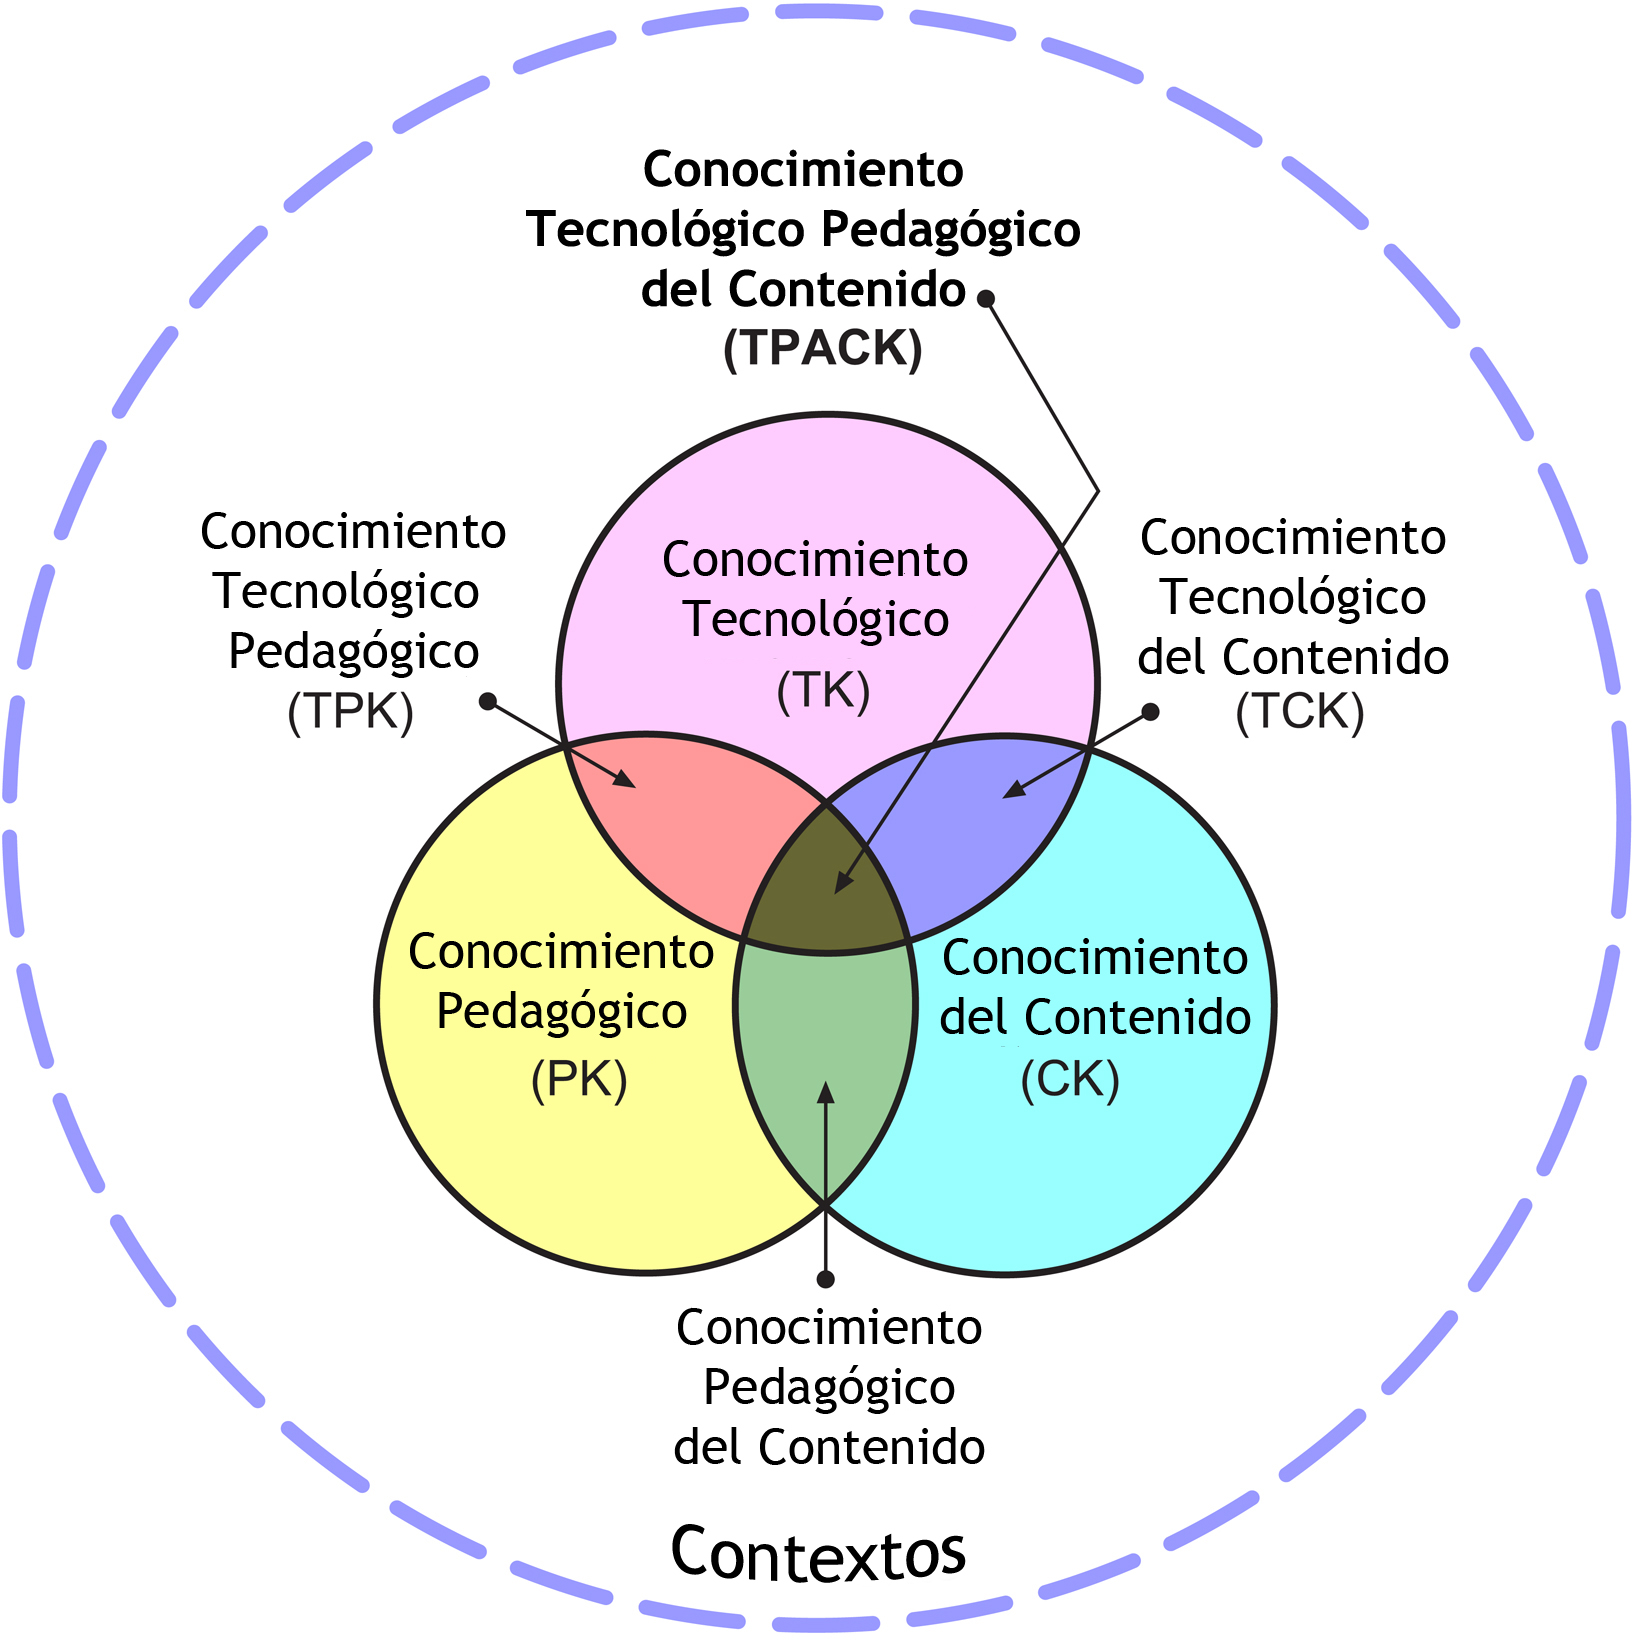
\includegraphics[width=0.85\textwidth]{fig-001.jpeg.jpeg}
 \caption{Dominios del modelo TPACK.}
 \label{fig01}
 \source{\url{http://www.tpack.org}}
\end{figure}

Según \textcite[p. 1610]{khine_exploring_2017} una de las limitaciones en las investigaciones TPACK es que los investigadores no consideran el contexto, lo que conlleva a que el conocimiento del contenido no sea articulado con claridad \cite{chai_validating_2013,voogt_technological_2013}. Esta limitación es considerable dado que el PCK depende del contexto y la materia \cite{shulman_those_1986,shulman_knowledge_1987}. Al considerar el panorama educativo en América Latina, se evidencian diferencias importantes en las características del mercado educativo, calidad de programas ofrecidos y arreglos institucionales \cite[p. 99]{gamboa_existen_2016}, además, diferencias en el contexto incluso dentro de una misma región \cite[p. 3]{tomaselli_pobreza_2014}, por consiguiente, es importante verificar la validez del cuestionario TPACK utilizado para este estudio.

\subsection{Conocimiento tecno-pedagógico}\label{sec-fmt-manuscrito}
Si bien, es necesario que los docentes tengan competencias TIC para incorporar las tecnologías en la práctica educativa \cite{suarez_rodriguez_competencias_2013}, también deben tener manejo pedagógico y de contenido.

El conocimiento disciplinar (CK) es la teoría que se estudia y transfiere a la práctica \cite[p. 7]{senge_quinta_1996}. Este constructo es el que menos se ha tomado en cuenta en el modelo TPACK, debido a que se espera que un docente se forme en profundidad en su disciplina, sin embargo, dichas competencias disciplinares pueden enriquecerse u olvidarse dependiendo del compromiso del docente \cite[p. 110]{cejas_leon_competencias_2016}. Por su parte, el conocimiento pedagógico (PK) es independiente a la disciplina, por lo que todo docente debe ser competente en el diseño del aprendizaje, planificación y orientación, contribuyendo en la mejora educativa y convirtiéndose en un agente de cambio \cite[p. 112]{cejas_leon_competencias_2016}.

Las competencias pedagógicas suelen ser inferiores a las competencias tecnológicas, lo que provoca limitaciones en la integración de las TIC en ambientes de aprendizaje, ya que se reproducen metodologías tradicionales para la utilización de estos recursos \cite{cabero_formacion_2014,suarez_rodriguez_competencias_2013}. Para que las TIC puedan ser integradas al proceso educativo, el docente deberá poseer competencias tecnológicas y pedagógicas, siendo la combinación de ambas la que llevará a una experiencia de aprendizaje exitosa \cite[107]{cejas_leon_competencias_2016}.

\section{Metodología}\label{sec-formato}
\subsection{Método}
Este estudio de desarrolló desde una metodología con un enfoque mixto. Es cuantitativa porque buscó establecer la existencia de diferencias entre el TPACK de los docentes en contexto de pandemia con el contexto de prepandemia. Es cualitativa porque consideró como técnica las nubes de palabras para el análisis de contenido, lo que permitió interpretar y comprender los objetivos priorizados propuestos por el Mineduc.

El diseño fue de tipo no experimental longitudinal, pues el TPACK de los docentes fue medido en 2018 y nuevamente medido a finales de 2020 y principio de 2021 para un análisis comparativo. Las variables fueron medidas sin ser manipuladas por los investigadores, por lo que la posición fue pasiva. De manera específica, este estudio tuvo como objetivo describir las variables del modelo TPACK y comparar los dominios de este modelo en contexto de prepandemia y pandemia relacionándolos con los objetivos priorizados.

\subsection{Participantes}\label{sec-modelo}
Bajo el contexto de emergencia sanitaria, se seleccionaron docentes de diversos establecimientos los que, además, participaron en el estudio IDETTED (Investigación, Desarrollo y Transferencia en Tecnologías de la Educación) realizado por la Universidad de Concepción en la región del Biobío, Chile, en el año 2018. Por lo tanto, la muestra fue no probabilística. Finalmente, la muestra quedó conformada por 178 profesores en servicio de distintas disciplinas y niveles. Estos docentes fueron contactados a través de redes sociales y vía correo electrónico.

\subsection{Procedimiento}\label{sec-organizacao}
Los datos fueron recopilados entre noviembre de 2020 y enero de 2021 a través de un cuestionario TPACK, el que se aplicó de manera virtual. Este incluyó una encuesta demográfica con los siguientes ámbitos: (1) años de experiencia, (2) grados académicos (Licenciatura, Maestría, Doctorado) y (3) tipo de institución educativa (pública, subvencionada, privada, otros). Los profesores accedieron al sitio web \url{http://www.sacited.cl/encuesta/} (accedido entre el 10 de diciembre de 2021 al 10 de enero de 2021). Para el resguardo ético de este estudio, los participantes firmaron un consentimiento informado previo a la aplicación del cuestionario.

Por otra parte, se seleccionaron las priorizaciones curriculares de Matemática \cite{unidad_de_curriculum_y_evaluacion_uce_priorizacion_2020b}, Lenguaje \cite{unidad_de_curriculum_y_evaluacion_uce_priorizacion_2020c}, Ciencias \cite{unidad_de_curriculum_y_evaluacion_uce_priorizacion_2020d} e Historia \cite{unidad_de_curriculum_y_evaluacion_uce_priorizacion_2020e} para generar nubes de palabras utilizando la página web \url{https://www.nubedepalabras.es} que permite limpiar los datos, arregla fuentes y generar imágenes de forma gratuita.

\subsection{Recopilación de la información}\label{sec-organizacao-latex}
\subsubsection{Cuestionario TPACK}
Este cuestionario se conformó por 35 ítems que determinan información de cada dominio del modelo TPACK: TK (7 ítems), CK (3 ítems), PK (7 ítems), PCK (4 ítems), TCK (4 ítems), TPK (5 ítems), y TPACK (5 ítems). Tiene una construcción tipo Likert de cinco opciones: “Muy en desacuerdo”, “En desacuerdo”, “Ni en de acuerdo, ni en desacuerdo”, “De acuerdo” y “Muy de acuerdo”. 

A pesar de que el cuestionario está validado en la provincia del Elqui, Chile, con un Alpha de Cronbach superior a 0.875 en todos los dominios \cite{tapia_silva_conocimiento_2019}, se realizó una validación para los docentes chilenos de la región del Biobío en contexto de pandemia, debido a que las diferencias contextuales pueden alterar los resultados del cuestionario TPACK \cite[p. 1618]{khine_exploring_2017}.

\section{Nubes de palabras}\label{sec-titulo}
La visualización de la información se utiliza para un análisis rápido en un contexto específico, por lo que la representación visual de palabras es útil para indicar las palabras más frecuentes en un texto y conocer donde se enfatiza un tema \cite[p. 78]{de_lucia_castillo_nubes_2016}. Las Nubes de Palabras combinan varios tamaños de fuentes en una sola imagen que agrupa palabras según su frecuencia \cite[p. 49]{viegas_timelinestag_2008}, las que presentan una descripción visual de un texto \cite[p. 634]{mcnaught_using_2010}. Pueden utilizarse para análisis pues es flexible y eficaz, pudiendo presentar de forma rápida una visión general de los términos más destacados de un texto \cite[p. 82]{de_lucia_castillo_nubes_2016}. 

\subsection{Análisis de la información}\label{sec-autores}
Para el estudio TPACK se utilizaron las pruebas de U Mann-Whitney y Kruskal Wallis para muestras independientes con el fin de comparar los resultados del cuestionario tomado en 2018 (contexto de prepandemia) con el cuestionario tomado en 2020-2021 (contexto de pandemia) y comparar los datos demográficos obtenidos (género, trayectoria académica y dependencia). Para ello se utilizó el software JASP para el análisis de datos.

Para las nubes de palabras, se generaron las imágenes de acuerdo con las priorizaciones curriculares para luego realizar un análisis descriptivo e interpretativo sustentado en la frecuencia de palabras, relacionándolo con los resultados de TPACK.

\section{Resultados}\label{sec-idioma}
\subsection{Validación del instrumento TPACK}
No hubo datos perdidos, por lo que toda la muestra contestó debidamente el cuestionario TPACK. El conocimiento tecnológico (TK) es la dimensión que obtuvo el promedio más bajo con un valor de 3,075 mientras que el conocimiento pedagógico de contenido (PCK) obtuvo el promedio de mayor valor con 3,636 siendo la diferencia entre ambos es de 0,561 puntos. Los datos más homogéneos son de la dimensión PCK con una desviación estándar de 0,425 mientras que los datos más dispersos son de la dimensión TCK con una desviación estándar de 0,606. A continuación, se detallan los resultados del cuestionario TPACK aplicado a la muestra de 178 docentes en contexto de pandemia, la validación del instrumento y comparación de grupos.

En primera instancia, se calculó el Alpha de Cronbach a todo el cuestionario, donde se identificó un valor de 0,96. Seguidamente, se realizó el mismo cálculo para cada una de las dimensiones del TPACK, donde todas obtuvieron un valor α de Cronbach superior a 0,8 tal como se muestra en la \Cref{tab01}, por lo que se afirma que el instrumento tiene una alta fiabilidad. 

\begin{table}[h!]
\centering
\begin{threeparttable}
\caption{Alpha de Cronbach por dimensión.}
\label{tab01}
\centering
\begin{tabular}{*{7}{S}}
\toprule
{TK} & {CK} & {PK} & {PCK} & {TCK} & {TPK} & {TPACK} \\
\midrule
$\alpha$ 0,867 & $\alpha$ 0,827 & $\alpha$ 0,861 & $\alpha$ 0,861 & $\alpha$ 0,920 & $\alpha$ 0,881 & $\alpha$ 0,925 \\
%$\alpha~0,867$ & $\alpha~0,827$ & $\alpha~0,861$ & $\alpha~0,861$ & $\alpha~0,920$ & $\alpha~0,881$ & $\alpha~0,925$ \\
\bottomrule
\end{tabular}
\source{Elaboración propia.}
\end{threeparttable}
\end{table}

\subsection{TPACK en contexto de pandemia}\label{sec-resumo}
En este apartado se caracterizan los resultados TPACK de docentes en contexto de pandemia, analizando la correlación entre los constructos y las diferencias por género, trayectoria académica y dependencia institucional.

\subsubsection{Análisis correlacional}\label{sec-secoes}
Se realizó el test de Kaiser Meyer y Olkin cuyo resultado obtenido fue de 0,866, por lo que se establece que existe relación entre las dimensiones del TPACK. Por su parte, la prueba de esfericidad de Bartlett arroja un valor p <0,001, por lo que se rechaza la hipótesis nula y se establece que existe relación significativa entre las dimensiones. La \Cref{tab02} presenta los resultados del coeficiente de correlación de Pearson entre las dimensiones del TPACK.

%TEm um erro na quantidade de colunas. rever.

\begingroup
\setlength\tabcolsep{4.5pt} % default value: 6pt
\begin{table}[h!]
\centering
\begin{threeparttable}
\caption{Correlación de Pearson entre dimensiones TPACK.}
\label{tab02}
\centering
\begin{tabular}{ll*{7}{S}}
\toprule
Variable & & TK & CK & PK & PCK & TCK & TPK & TPACK \\
\midrule
\arrayrulecolor[gray]{.7}
\multirow{2}{*}{TK} & R de Pearson & \text{--} & & & & & \\
%\cmidrule{2-9}
 & Valor p & 0,359 & \text{--} & & & & & \\
 \midrule
\multirow{2}{*}{CK} & R de Pearson & 0,359 & \text{--} & & & & \\
%\cmidrule{2-9}
 & Valor p & <0,001 & \text{--} & & & & \\
 \midrule
 \multirow{2}{*}{PK} & R de Pearson & 0,426 & 0,677 & \text{--} & & & & \\
%\cmidrule{2-9}
 & Valor p & <0,001 & <0,001 & \text{--} & & & & \\
 \midrule
\multirow{2}{*}{PCK} & R de Pearson & 0,358 & 0.524 & 0,745 & \text{--} & & & \\
%\cmidrule{2-9}
 & Valor p & <0,001 & <0,001 & <0,001 & \text{--} & & & \\
 \midrule
\multirow{2}{*}{TCK} & R de Pearson & 0,722 & 0,409 & 0,533 & 0,485 & \text{--} & & \\
%\cmidrule{2-9}
 & Valor p & <0,001 & <0,001 & <0,001 & <0,001 & \text{--} & & \\
\midrule
\multirow{2}{*}{TPK} & R de Pearson & 0,664 & 0,450 & 0,561 & 0,526 & 0,804 & \text{--} & \\
%\cmidrule{2-9}
 & Valor p & <0,001 & <0,001 & <0,001 & <0,001 & <0,001 & \text{--} & \\
\midrule
\multirow{2}{*}{TPACK} & R de Pearson & 0,699 & 0,423 & 0,551 & 0,518 & 0,868 & 0,804 & \text{--} \\
%\cmidrule{2-9}
& Valor p & <0,001 & <0,001 & <0,001 & <0,001 & <0,001 & <0,001 & \text{--} \\
\arrayrulecolor{black}
\bottomrule
\end{tabular}
\source{Elaboración propia.}
\end{threeparttable}
\end{table}
\endgroup

Se observó una correlación baja entre las dimensiones CK – TK y PCK – TK, mientras que las dimensiones PK – TK, PCK – CK, TCK – CK, TCK – PK, TCK – PCK, TPK – CK, TPK – PK, TPK – PCK, TPACK – CK, TPACK – PK y TPACK – PCK presentaron una correlación moderada. Las dimensiones PK – CK, PCK – PK, TCK – TK, TPK – TK y TPACK – TK presentaron una correlación alta mientras que existe una correlación muy alta entre las dimensiones TPK – TCK, TPACK – TCK y TPACK – TPK.

\subsubsection{Comparación de grupos: Género }\label{sec-format-simple}
Para un estudio demográfico de TPACK, se separó la muestra según género donde participaron 63 hombres y 115 mujeres. Se aplicó el Test de U de Mann - Whitney para comparar el TPACK de estos dos grupos. Tal como se muestra en la \Cref{tab03}, no se presentan valores p significativos en ningún componente TPACK, por lo que no existe diferencia significativa entre los resultados TPACK de hombres y mujeres.

\begin{table}[h!]
\centering
\begin{threeparttable}
\caption{Comparación entre TPACK hombres y mujeres.}
\label{tab03}
\centering
\begin{tabular}{lSS}
\toprule
Variable & W & p \\
\midrule
TK & 4131,000 & 0,121 \\
CK & 3845,000 & 0,480 \\
PK & 3501,000 & 0,711 \\
PCK & 3867,500 & 0,429 \\
TCK & 3677,500 & 0,864 \\
TPK & 3779,000 & 0,631 \\ 
TPACK & 3992,000 & 0,252 \\ 
\bottomrule
\end{tabular}
\source{Elaboración propia.}
\end{threeparttable}
\end{table}

\subsubsection{Trayectoria académica}\label{sec-links}
Tomando los años de experiencia y grados académicos, se separó la muestra según trayectoria académica. Como guía, se tomó los tramos y progresión de la carrera docente modificando algunos aspectos. A los años de experiencia se fue sumando 2 puntos por diplomado, 4 puntos por magister y 8 puntos por doctorado. Finalmente, la trayectoria académica se separó en los tramos de Inicial (0 a 3 puntos) con 31 docentes, Temprano (4 a 7 puntos) con 30 docentes, Avanzado (8 a 11 puntos) con 39 docentes, Experto I (12 a 15 puntos) con 26 docentes y Experto II (16 o más puntos) con 52 docentes.

Se aplicó el Test de Kruskal Wallis, donde solo se presenta un valor p significativo en el componente TPK. Para saber las diferencias, se realizó una prueba de Post Hoc de Games Howell para datos no paramétricos, cuyos resultados se presentan en la \Cref{tab04}.

\begin{table}[h!]
\centering
\begin{threeparttable}
\caption{Prueba Post Hoc de Games-Howell para Comparación – TPK.}
\label{tab04}
\centering
\begin{tabular}{l*{5}{S}}
\toprule
Comparación & {Diferencia de medias} & {SE} & {t} & {df} & {P tukey} \\
\midrule
AVANZADO - EXPERTO I  & 0,390 & 0,126 & 3,094 & 58,537 & <0,05 \\ 
AVANZADO - EXPERTO II & 0,372 & 0,138 & 2,707 & 67,292 & 0,063 \\ 
AVANZADO - INICIAL & 0,152 & 0,125 & 1,216 & 53,868 & 0,742 \\
AVANZADO - TEMPRANO & 0,136 & 0,113 & 1,203 & 68,765 & 0,749 \\
EXPERTO I - EXPERTO II & -0,018   & 0,142 & -0,127 & 66,983 & 1,000 \\ 
EXPERTO I - INICIAL & -0,238 & 0,129 & -1,843 & 53,833 & 0,360 \\ 
EXPERTO I - TEMPRANO & -0,254 & 0,118 & -2,145 & 63,358 & 0,214 \\ 
EXPERTO II - INICIAL & -0,221 & 0,141 & -1,569 & 62,903 & 0,523 \\ 
EXPERTO II - TEMPRANO & -0,236 & 0,130 & -1,808 & 70,769 & 0,377 \\ 
INICIAL - TEMPRANO & -0,015 & 0,117 & -0,131 & 57,022 & 1,000 \\ 
\bottomrule
\end{tabular}
\source{Elaboración propia.}
\end{threeparttable}
\end{table}

Los resultados revelan que el grupo de docentes en tramo avanzado tiene una percepción sobre su conocimiento pedagógico tecnológico significativamente superior al grupo de docentes en tramo Experto I.

\subsubsection{Dependencia institucional}\label{sec-outras-estr}
Se separó la muestra según el tipo de dependencia académica donde los docentes se desempeñan: municipal con 71 docentes, subvencionado con 70 docentes, particular con 24 docentes y otras (DAEM, JUNJI o universidades) con 13 docentes.

Se aplicó el Test de Kruskal Wallis para comparar los componentes del TPACK de estos grupos. La \Cref{tab05} muestra que no se presentan valores p significativos en ninguno de los componentes TPACK, por lo que no existe diferencia entre la dependencia instituciones de los docentes para ninguno de los componentes del TPACK.

\begin{table}[h!]
\centering
\begin{threeparttable}
\caption{Comparación entre TPACK según dependencia.}
\label{tab05}
\centering
\begin{tabular}{l*{3}{S}}
\toprule
Factor & {Estadístico} & {df} & {p} \\
\midrule
TK & 6,673 & 3 & 0,083 \\ 
CK & 4,775 & 3 & 0,189 \\
PK & 5,208 & 3 & 0,157 \\
PCK & 0,464 & 3 & 0,927 \\
TCK & 5,633 & 3 & 0,131 \\
TPK & 2,246 & 3 & 0,523 \\
TPACK & 3,396 & 3 & 0,335 \\
\bottomrule
\end{tabular}
\source{Elaboración propia.}
\end{threeparttable}
\end{table}


\subsection{Cambios en contexto de pandemia}\label{sec-listas}
Este apartado da cuenta de las diferencias entre los grupos de docentes en contexto de prepandemia y contexto de pandemia. Además, analiza los textos ministeriales de los objetivos priorizados en las áreas de matemática, lenguaje, historia y ciencias.

\subsubsection{TPACK de docentes en contexto de Prepandemia y Pandemia }\label{sec-figuras-tabelas}
Se tomo la muestra 178 profesores en 2020-2021 (grupo 1) a quienes se les aplicó el cuestionario TPACK en contexto de pandemia para compararlo con el grupo de 289 profesores de 2018 (grupo 2) a quienes se les aplicó dicho cuestionario en contexto de prepandemia.

Se realizaron dos comparaciones de grupo utilizando el estadígrafo U de Mann Whitney, estableciendo en el primer caso las siguientes hipótesis: H0 = No existe diferencia entre ambos grupos; H1 = Existe diferencia entre ambos grupos, donde Grupo 1 > Grupo 2. La \Cref{tab06} presenta los resultados de la aplicación del estadígrafo.

\begin{table}[h!]
\centering
\begin{threeparttable}
\caption{Comparación donde el grupo 1 es mayor al grupo 2.}
\label{tab06}
\centering
\begin{tabular}{l*{2}{S}}
\toprule
Variable & {W} & {p} \\
\midrule
TK & 29441,000 & < 0,005 \\	
CK & 23777,000 & 0,929 \\
PK & 19999,000 & 1,000 \\
PCK & 23397,000 & 0,963 \\
TCK & 23044,500 & 0,974 \\
TPK & 23233,000 & 0,963 \\
TPACK & 24611,500 & 0,788 \\
\bottomrule
\end{tabular}
\source{Elaboración propia.}
\end{threeparttable}
\end{table}

El único caso donde se rechaza la hipótesis nula y se acepta la hipótesis alternativa con un 99,5\% de confianza es para TK, donde existe una diferencia entre ambos grupos siendo el grupo de docentes en contexto de pandemia quienes consideran tener un mayor conocimiento tecnológico que los profesores en contexto de prepandemia.

En el segundo caso las siguientes hipótesis son las siguientes: H0 = No existe diferencia entre ambos grupos; H1 = Existe diferencia entre ambos grupos, donde Grupo 1 < Grupo 2. La \Cref{tab07} presenta los resultados de la aplicación del estadígrafo.

\begin{table}[h!]
\centering
\begin{threeparttable}
\caption{Comparación donde el grupo 1 es menor al grupo 2.}
\label{tab07}
\centering
\begin{tabular}{l*{2}{S}}
\toprule
Variable & {W} & {p} \\
\midrule
TK & 29441,000 & 0,996 \\
CK & 23777,000 & 0,071 \\
PK & 19999,000 & <0,001 \\
PCK & 23397,000 & < 0,05 \\
TCK & 23044,500 & < 0,05 \\
TPK & 23233,000 & < 0,05 \\
TPACK & 24611,500 & 0,212 \\
\bottomrule
\end{tabular}
\source{Elaboración propia.}
\end{threeparttable}
\end{table}

Con un 95\% de confianza, se rechaza la hipótesis nula y se acepta la alternativa en los casos de PCK, TCK y TPK, por lo que existe diferencia entre ambos grupos. Los docentes en contexto de pandemia consideran tener un menor conocimiento pedagógico del contenido, conocimiento tecnológico del contenido y conocimiento tecnológico pedagógico que los docentes en contexto de prepandemia. De esta misma manera, con un 99,9\% de confianza, se rechaza la hipótesis nula y se acepta la hipótesis alternativa para PK, es decir, los docentes en contexto de pandemia consideran tener un menor conocimiento pedagógico que los docentes en contexto de prepandemia.

\subsubsection{Objetivos Priorizados}\label{sec-quotesandfootnotes}
Se generaron cuatro nubes de objetivos priorizados de primero básico a cuarto medio de las asignaturas Matemática, Lenguaje, Historia y Ciencias. Las \Cref{fig2a}, \Cref{fig2b}, \Cref{fig2c} y \Cref{fig2d} presentan las nubes generadas a partir de los objetivos priorizados.

\begin{figure}[htbp]
 \centering
 \begin{minipage}{.45\textwidth}
 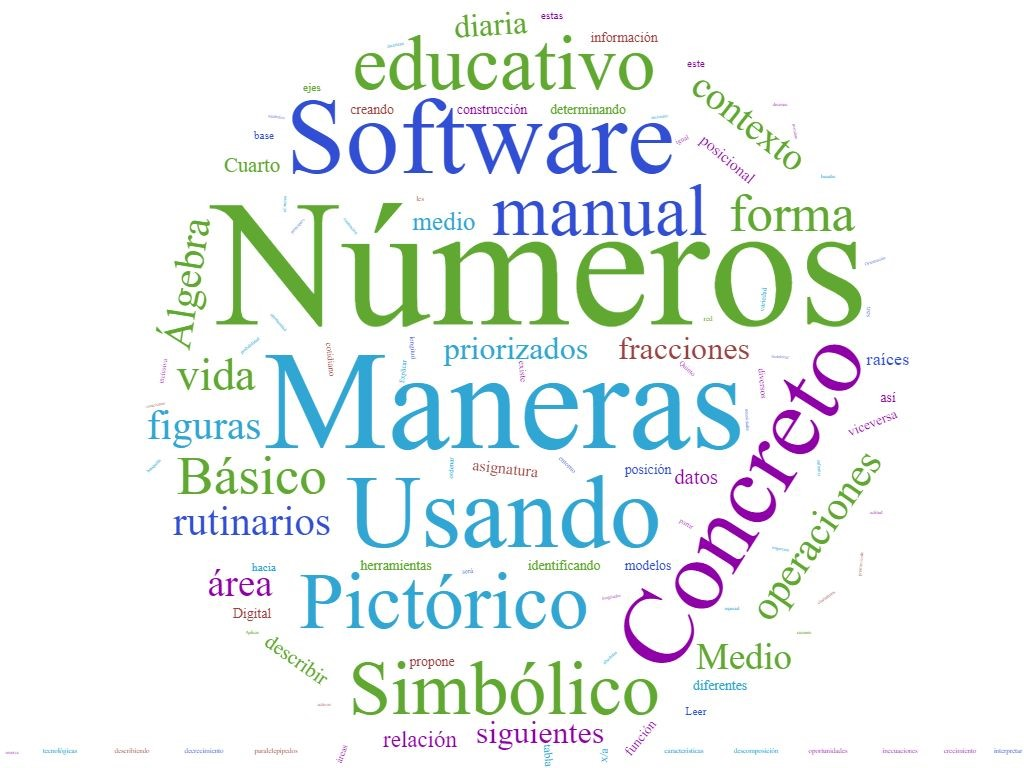
\includegraphics[width=\textwidth]{fig-002a.jpeg.jpg}
 \caption{Nubes de palabras de objetivos priorizados en (a) Matemática.}
 \label{fig2a}
 \source{Elaboración propia.}
 \end{minipage}%
 \qquad
 \begin{minipage}{0.45\textwidth}
 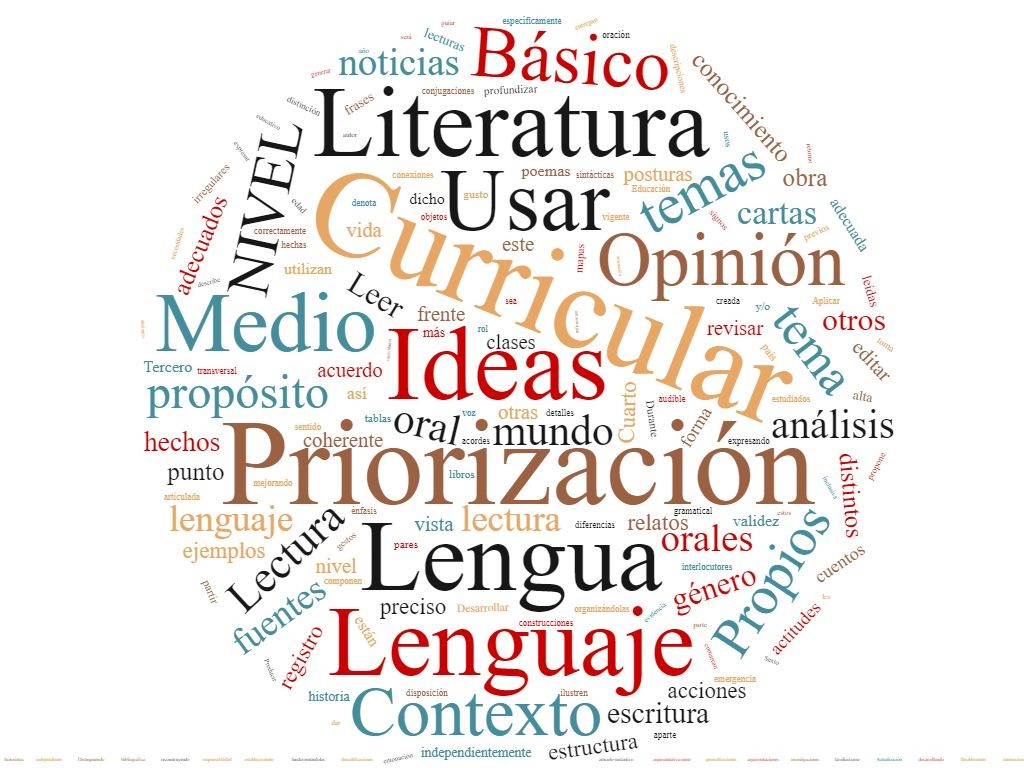
\includegraphics[width=\textwidth]{fig-002b.jpeg.jpg}
 \caption{Nubes de palabras de objetivos priorizados en (b) Lenguaje.}
 \label{fig2b}
 \source{Elaboración propia.} 
 \end{minipage}%
\end{figure}

\begin{figure}[htbp]
 \centering
 \begin{minipage}{.45\textwidth}
 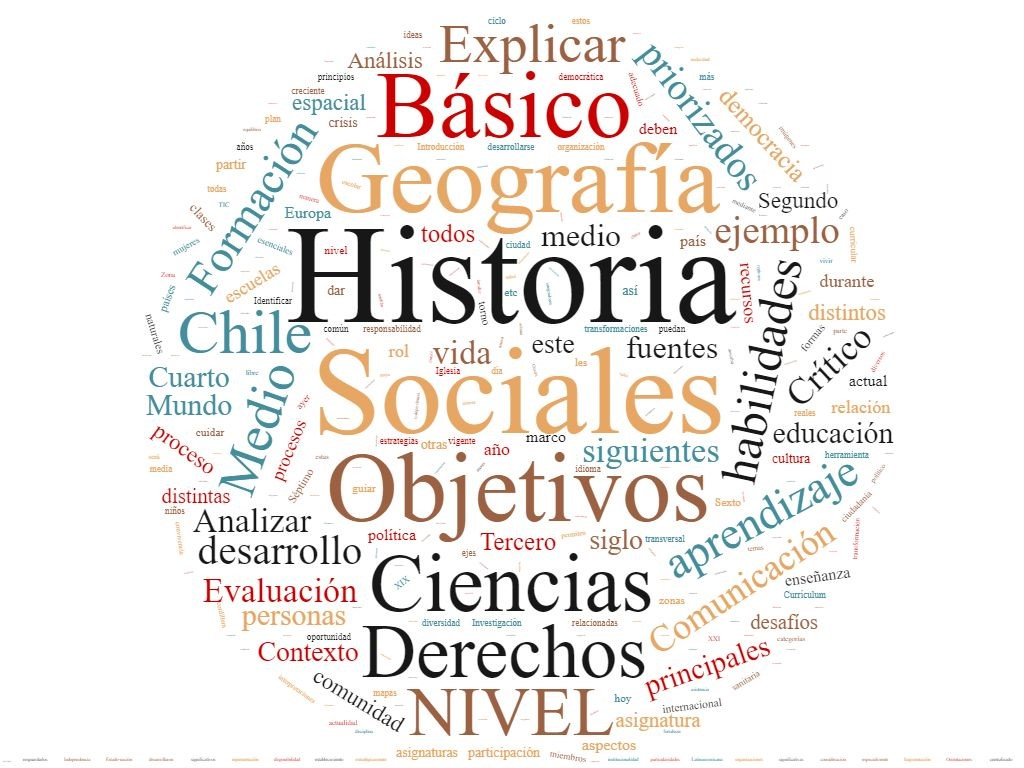
\includegraphics[width=\textwidth]{fig-002c.jpeg.jpg}
 \caption{Nubes de palabras de objetivos priorizados en (c) Historia.}
 \label{fig2c}
 \source{Elaboración propia.}
 \end{minipage}%
 \qquad
 \begin{minipage}{0.45\textwidth}
 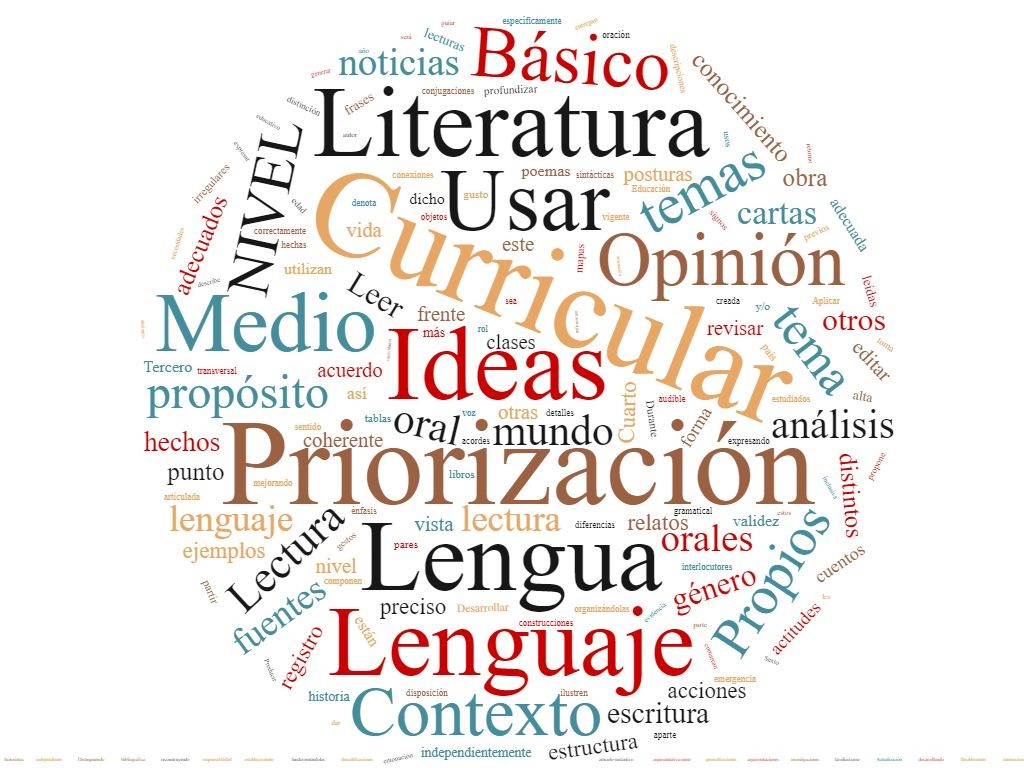
\includegraphics[width=\textwidth]{fig-002b.jpeg.jpg}
 \caption{Nubes de palabras de objetivos priorizados en (d) Ciencias Naturales.}
 \label{fig2d}
 \source{Elaboración propia.} 
 \end{minipage}%
\end{figure}

Se aprecia en la nube de palabras de Matemática que la palabra más frecuente es “Números”. También se encuentran palabras como “Manera”, “Usando”, “Concreto”, “Pictórico”, “Simbólico” y “Software”. En menor medida se aprecian las palabras “Vida”, “Rutinarios”, “Contexto” y “Diario”. 

En lenguaje las palabras más frecuentes son “Literatura”, “Lengua” y “Lenguaje”. Las palabras “Opinión”, “Medio” y “Análisis” aparecen medianamente. En menor medida se observan las palabras “Hechos”, “Mundo”, “Contexto” y “Noticias”. 

En historia las palabras más frecuentes son “Geografía”, “Historia” y “Derechos”. También se evidencian las palabras “Comunicación”, “Analizar” y “Explicar”. Con menor frecuencia las palabras “Crítico”, “Mundo”, “Contexto” y “Comunidad”. 

Finalmente, en los objetivos priorizados de Ciencias las palabras más frecuentes son “Explicar”, “Analizar” y “Comprensión”. En menor frecuencia se evidencian las palabras “Natural”, “Química” y “Cuerpo”.

\section{Discusión}\label{sec-equacao}
Antes de comenzar la discusión es importante destacar que existe una alta fiabilidad del instrumento aplicado con un Alpha de Cronbach similar a la de \textcite{tapia_silva_conocimiento_2019}, validando el instrumento para el contexto en donde fue aplicado el cuestionario TPACK.

Con respecto a los docentes, se advierte que presentan resultados heterogéneos en su percepción TPACK, donde las dimensiones que no incluyen en el conocimiento tecnológico (CK, PK y PCK) presentan una mayor media y menor desviación estándar que aquellas que si incluyen este conocimiento (TK, TCK, TPK y TPACK). Este resultado es idéntico al encontrado por \textcite{tapia_silva_conocimiento_2019}.

Por otra parte, existe correlación entre las dimensiones del TPACK, donde se evidencia que la alta relación entre el TPACK y las otras dimensiones requiere de un conocimiento TIC mayor. La baja relación entre CK – TK y PCK – TK evidencian la poca vinculación entre la tecnología con la pedagogía y el contenido. Respecto al conocimiento tecnológico pedagógico (TPK) existen diferencias entre los docentes según su trayectoria académica, la diferencia más significativa está entre los docentes en tramo avanzado y experto I donde los docentes avanzados tienen mejor puntaje de autopercepción. Estos resultados coinciden con las investigaciones de \textcite{castera_self-reported_2020,ladron-de-guevara_moreno_conocimiento_2019}. 

El grupo de profesores que participó en el estudio en 2018 con el grupo que participó en el estudio de 2020-2021 tienen diferencias en las dimensiones TK, PCK, TCK, TPK y PK. En contexto de pandemia, los docentes se perciben con mayor conocimiento tecnológico que en contexto de prepandemia. En los estudios de \textcite{arevalo_duarte_competencias_2016,silva_teachers_2019,tapia_silva_conocimiento_2019} hechos antes de la pandemia, los docentes tienen un TK más bajo en comparación a las otras dimensiones, sin embargo, en esta investigación todas las dimensiones tienen resultados similares en sus promedios, siendo todos sobre 3 puntos. Este aumento concuerda con los resultados de \textcite[p. 12]{rocha_estrada_docentes_2022} quienes afirman que los docentes en contexto de pandemia se adaptaron fácilmente al uso tecnológico, asimismo, \textcite[p. 28]{anderete_schwal_pandemia_2021} afirma que los docentes pudieron adaptar y utilizar las TIC que tenían disponibles, como Whatsapp, para lograr comunicación y resultados con sus estudiantes.

A diferencia de lo anterior, los docentes en contexto de pandemia se sienten con menor conocimiento pedagógico que los docentes en contexto prepandémico, lo que puede deberse a la priorización curricular o a la adaptación de actividades al contexto de hogar. Esta idea se refuerza con lo declarado por \textcite{cabero_formacion_2014,suarez_rodriguez_competencias_2013} quienes afirman que las competencias tecnológicas suelen ser superiores a las competencias pedagógicas, lo que conlleva a aplicar metodologías tradicionales aun cuando se utilicen recursos tecnológicos.

Pese a las discrepancias encontradas, una mirada general revela que los docentes se perciben con un alto nivel en todas las dimensiones TPACK, el decir, sienten que tienen un alto conocimiento tecnológico, pedagógico, de contenido y las combinaciones entre estas. Esto coincide con los resultados obtenidos por el \textcite{ministerio_de_educacion_mineduc_docentes_2016} relacionados con la alta percepción de los docentes en la integración de las TIC para uso pedagógico. Sin embargo, estos hallazgos no coinciden con los bajos resultados del manejo tecnológico encontrados por \textcite{agencia_de_calidad_de_la_education_ace_estudio_2018} y con los resultados obtenidos en otros estudios similares, donde se evidencian que los docentes en contexto de pandemia tienen un bajo conocimiento tecnológico relacionado a la educación \cite{fernandez-chavez_early_2022,salcedo-lagos_teachers_2021}. 

Por otra parte, no existe diferencia del TPACK entre hombres y mujeres, al igual que en los estudios de \textcite{bakar_mathematics_2020,castera_self-reported_2020}, de igual modo, no existe diferencia según la dependencia institucional. Sin embargo, los resultados del análisis de Kruskal Wallis presentan diferencias entre los grupos de docentes con diferentes trayectorias académicas para el TPK. Los docentes de tramo avanzado se perciben con un conocimiento pedagógico tecnológico significativamente superior a los docentes de los tramos Experto I. Esto se asocia a los resultados del estudio de \textcite{salcedo-lagos_teachers_2021}, donde claramente, los docentes en tramo avanzado tienen un mayor conocimiento sobre TIC en aula y en clases virtuales.

Según las nubes de palabras formadas por los objetivos priorizados, las palabras más frecuentes tienen relación con los contenidos y habilidades requeridas en las asignaturas correspondientes, como Natural, Literatura, Número, Geografía, Analizar, Comprender, Desarrollar, entre otras. En matemática se destaca la palabra Software, la única relacionada con TIC entre las asignaturas. En todos los objetivos priorizados se destacan palabras que se relacionan con el aprendizaje en el entorno, como Contexto, Mundo, Rutinarios, Comunidad, entre otras.

Los resultados muestran que la principal necesidad de los objetivos priorizados es la enseñanza de los contenidos en contexto y que propicien ciertas habilidades. Sin embargo, autores como \textcite{cabero_formacion_2014,cejas_leon_competencias_2016,suarez_rodriguez_competencias_2013} advierten que para integrar las TIC de forma efectiva al proceso educativo es necesario incorporarlas junto al contenido y a la pedagogía, es decir, que estas formen parte de los objetivos de aprendizaje, o en este caso, de los objetivos priorizados, cosa que no se evidencia en los textos ministeriales.

\section{Conclusiones}\label{sec-codigos}
A partir de las preguntas planteadas para esta investigación surgen las siguientes conclusiones:

\begin{enumerate}
    \item El cuestionario TPACK tiene una alta fiabilidad en este y otros estudios, por lo que es fiable su aplicación en otro contexto territorial e histórico.
    \item Los resultados TPACK no muestran diferencias significativas en cuanto a género y dependencia educacional. Respecto a la trayectoria académica los docentes en tramo avanzado muestran mayor autopercepción TPACK en comparación a los docentes experto I.
    \item Al considerar los resultados TPACK, los docentes chilenos se auto perciben con un mayor manejo tecnológico, pero con un menor manejo pedagógico, lo que pudiese estar relacionado con las necesidades de los objetivos priorizados, ya que consideran el contenido y su adaptación según el contexto, pero no la integración pedagógica de las tecnologías.
\end{enumerate}


\section{Limitaciones y Prospectivas}\label{sec-contributors-expl}
Este estudio no considera la misma muestra para realizar comparaciones, por lo que los resultados podrías mejorar rotundamente si se tomaran los mismos sujetos de muestra. Pese a esto, el análisis comparativo entre grupos diferentes es significativo y aporta conocimiento empírico sobre los cambios perceptivos de los docentes antes y después de la pandemia.

Se proyecta recoger datos con la misma muestra en contexto de post pandemia para verificar la permanencia y perspectiva y de conocimiento de los docentes al pasar por este periodo de emergencia sanitaria.

\section{Agradecimientos}\label{sec-conclusao}
Esta investigación se desarrolla en el marco del proyecto FONDECYT 1201572 (2020-2024): “Evaluación de la integración pedagógica de las tecnologías de la información y comunicación en el aula de matemática y de lenguaje y comunicación, desde el modelo TPACK basado en competencias”.


\printbibliography\label{sec-bib}
% if the text is not in Portuguese, it might be necessary to use the code below instead to print the correct ABNT abbreviations [s.n.], [s.l.]
%\begin{portuguese}
%\printbibliography[title={Bibliography}]
%\end{portuguese}


%full list: conceptualization,datacuration,formalanalysis,funding,investigation,methodology,projadm,resources,software,supervision,validation,visualization,writing,review
\begin{contributors}[sec-contributors]
\authorcontribution{Susan Rivera-Robles}[conceptualization,formalanalysis,investigation,methodology,validation,visualization,writing]
\authorcontribution{Pedro Salcedo-Lagos}[conceptualization,investigation,projadm,resources,software,validation,supervision,review]
\authorcontribution{Carolina Fernández-Chávez}[supervision,visualization,review]
\authorcontribution{María Graciela Badilla-Quintana}[projadm,supervision,review]
\end{contributors}

\end{document}

